%%%%%%%%%%%%%%%%%%%%%%%%%%%%%%%%%%%%%%%%%%%%%%%%%%
% NJU Thesis
% 南京大学毕业论文LaTeX模板
% Version 0.10.1 (2021-09-26)
%
% 请关注项目地址以获取最新变化
% https://github.com/nju-lug/NJUThesis
% https://git.nju.edu.cn/nju-lug/nju-latex-templates/njuthesis
% https://ctan.org/pkg/njuthesis
%
% 贡献者
% Yu XIONG @atxy-blip   Yichen ZHAO @FengChendian   
% Song GAO @myandeg     Chang MA @glatavento   
% Yilun SUN @HermitSun  Yinfeng LIN @linyinfeng
% 
% 许可证
% LaTeX Project Public License(版本 1.3c 或更高)
%
%%%%%%%%%%%%%%%%%%%%%%%%%%%%%%%%%%%%%%%%%%%%%%%%%%
\documentclass[
    customlatinfont=windows,% 设置英文字符集
    ]{hkustthesis}

% 设置个人信息
\hkustsetup {
    % 有空格的内容请用 {} 包裹
    % 注意不要有空行,否则可能报错
    info = {
        degree = {MPhil},
        % Thesis Title
        title = {A Brief Introduction to Writing Thesis with This \hologo{LaTeX} Template}, 
        % 关键词
        keywords = {Neon, Genesis, Evangelion},
        % 姓名学号
        grade = {2021},
        student-id = {20112233},
        author = {Cruel Angel},
        % 院系专业
        %school = {School of Engineering},
        department = {Department of NERV},
        major = {Human Instrumentality Project},
        field = {Nanophotonics},
        % 导师
        supervisor = {Adams},
        supervisor-title = {Prof.},
        % 第二导师,如无则留空
        co-supervisor = {Lilith},
        co-supervisor-title = {Prof.},
        % 提交日期
        submit-date = {October 2021}, % Only <month year>
        submit-date-long = {31 October 2021}, % <date month year>
        % 答辩,均为研究生项
        defend-date = {December 31 2021},
        chairman = {Prof. Ikari Gendo},
        depthead = {Prof. Ikari Yui},
        reviewer = {Prof. A, Prof. B, Prof. C, Prof. D (External Examiner)},
        city = {Geo Front},
    }
}

% 设置图片存储位置
\graphicspath{{figure/}}

% 导入参考文献数据
\addbibresource{mythesis.bib}

\begin{document}

%-------------------------------------------------
% Titlepage, Authorization, Signature
% (Preface), Acknowledgement
% TOC, List of Figures, List of Tables
% Abstract
%-------------------------------------------------

\frontmatter
\maketitle 
\authorization
\signaturepage

%\begin{preface}

\blindtext

\vspace{1cm}
\begin{flushright}
Author\\
2021. HK
\end{flushright}

\end{preface}

\begin{acknowledgements}

Thanks to \href{https://git.nju.edu.cn/nju-lug/lug-introduction}{NJU Linux User Group}.

\end{acknowledgements}


\tableofcontents
\listoffigures
\listoftables

\input{chapters/Abstract.tex}

%-------------------------------------------------
% Main body
%-------------------------------------------------
\mainmatter

\chapter{Introduction}

\section{Background}\label{chap:intro:sec:background}

\blindtext

Cite a paper \cite{test}.

\subsection{Enumitem}

Itemize.

\begin{itemize}
  \item Test test.
  \item Test test.
  \item Test test.
  \begin{itemize}
    \item test test
    \item test test\footnote{\blindtext}
    \item test test
    \item test test
  \end{itemize}
  \item Test test.
\end{itemize}

Enumerate.

\begin{enumerate}
  \item Test test.
  \item Test test.
  \item Test test.
  \begin{enumerate}
    \item test test
    \item test test\footnote{\blindtext}
    \item test test
    \item test test
  \end{enumerate}
  \item Test test.
\end{enumerate}


\chapter{Environments}

\section{Compile locally}

\subsection{Install \hologo{TeX} distribution}

\begin{table}[ht]
    \caption{Environments tested}
    % \label{tab:1}
    \begin{tabular}{ccc}
        \toprule
        OS & TeX & Test \\
        \midrule
        Windows 10 & \hologo{TeX}\,Live 2021 & Pass \\
        Windows 10 & \hologo{MiKTeX} & Pass \\
        Windows 10 & \hologo{TeX}\,Live 2020 & cref problem  \\
        macOS 10.15 & \hologo{TeX}\,Live 2021 & Pass \\
        Ubuntu 20.04 & \hologo{TeX}\,Live 2021 & Pass \\
        \bottomrule
    \end{tabular}
\end{table}

\subsection{Editor}

\verb|vscode| with \verb|LaTeX Workshop| is recommended.

\subsection{Compile toolchain}

\verb|latexmk -xelatex mythesis.tex|

\chapter{Layout}
\label{chap:layout}

\section{Coverpage}

\subsection{Format sample}

\blindtext
\chapter{Fig, table and Code}

\section{Code}

\subsection{Inline code}
Use \lstinline|\lstinline$<code>$| to print the code snippets. The exclamation marks delimit
the code and can be replaced by any character not in the code;
\lstinline|var i:integer;| gives the same result.

\section{Figure}

\begin{figure}[!htb]
  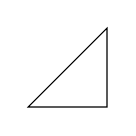
\begin{tikzpicture}
    \draw (0,0) -- (1, 0) -- (1, 1) -- cycle;
  \end{tikzpicture}
  \caption{An example tikz picture}
  \label{fig:tikz example}
\end{figure}

You can use \lstinline|\cref{}| to automatically setup the cross reference name; instead, you can always use \lstinline|\ref{}| to customize the appearence of the cross reference.

An example image is shown in \cref{fig:tikz example} or Figure (\ref{fig:tikz example}).

\chapter{Math}

\section{Symbols}

Caligraphic letters: $\mathcal{A}$ 

Mathbb letters: $\mathbb{A}$

Mathfrak letters: $\mathfrak{A}$

Math Sans serif letters: $\mathsf{A}$

Math bold letters: $\mathbf{A}$

Math bold italic letters: $\mathbi{A}$


\input{chapters/Conclusions.tex}

%-------------------------------------------------
%	参考文献
%-------------------------------------------------

\printbibliography[
    heading=bibintoc,% 插入目录条目
    title=References]

%-------------------------------------------------
%	附录部分
%-------------------------------------------------
\appendix

\input{chapters/Publications.tex}
\chapter{FYTGS~Requirements}
\label{chap:standard}

Requirements

\blindtext

\end{document}
